\documentclass{article}

\usepackage{graphicx}
\usepackage{tikz}
\usepackage{tikzsymbols}
\usetikzlibrary{calc,patterns,shapes.geometric}
\pagestyle{empty}
\usepackage[margin=0pt]{geometry}
\geometry{papersize={14in,12in}}

\def\centerarc[#1](#2)(#3:#4:#5){\draw[#1] ($(#2)+({#5*cos(#3)},{#5*sin(#3)})$) arc (#3:#4:#5);}

\begin{document}
	\begin{figure}
		\centering
		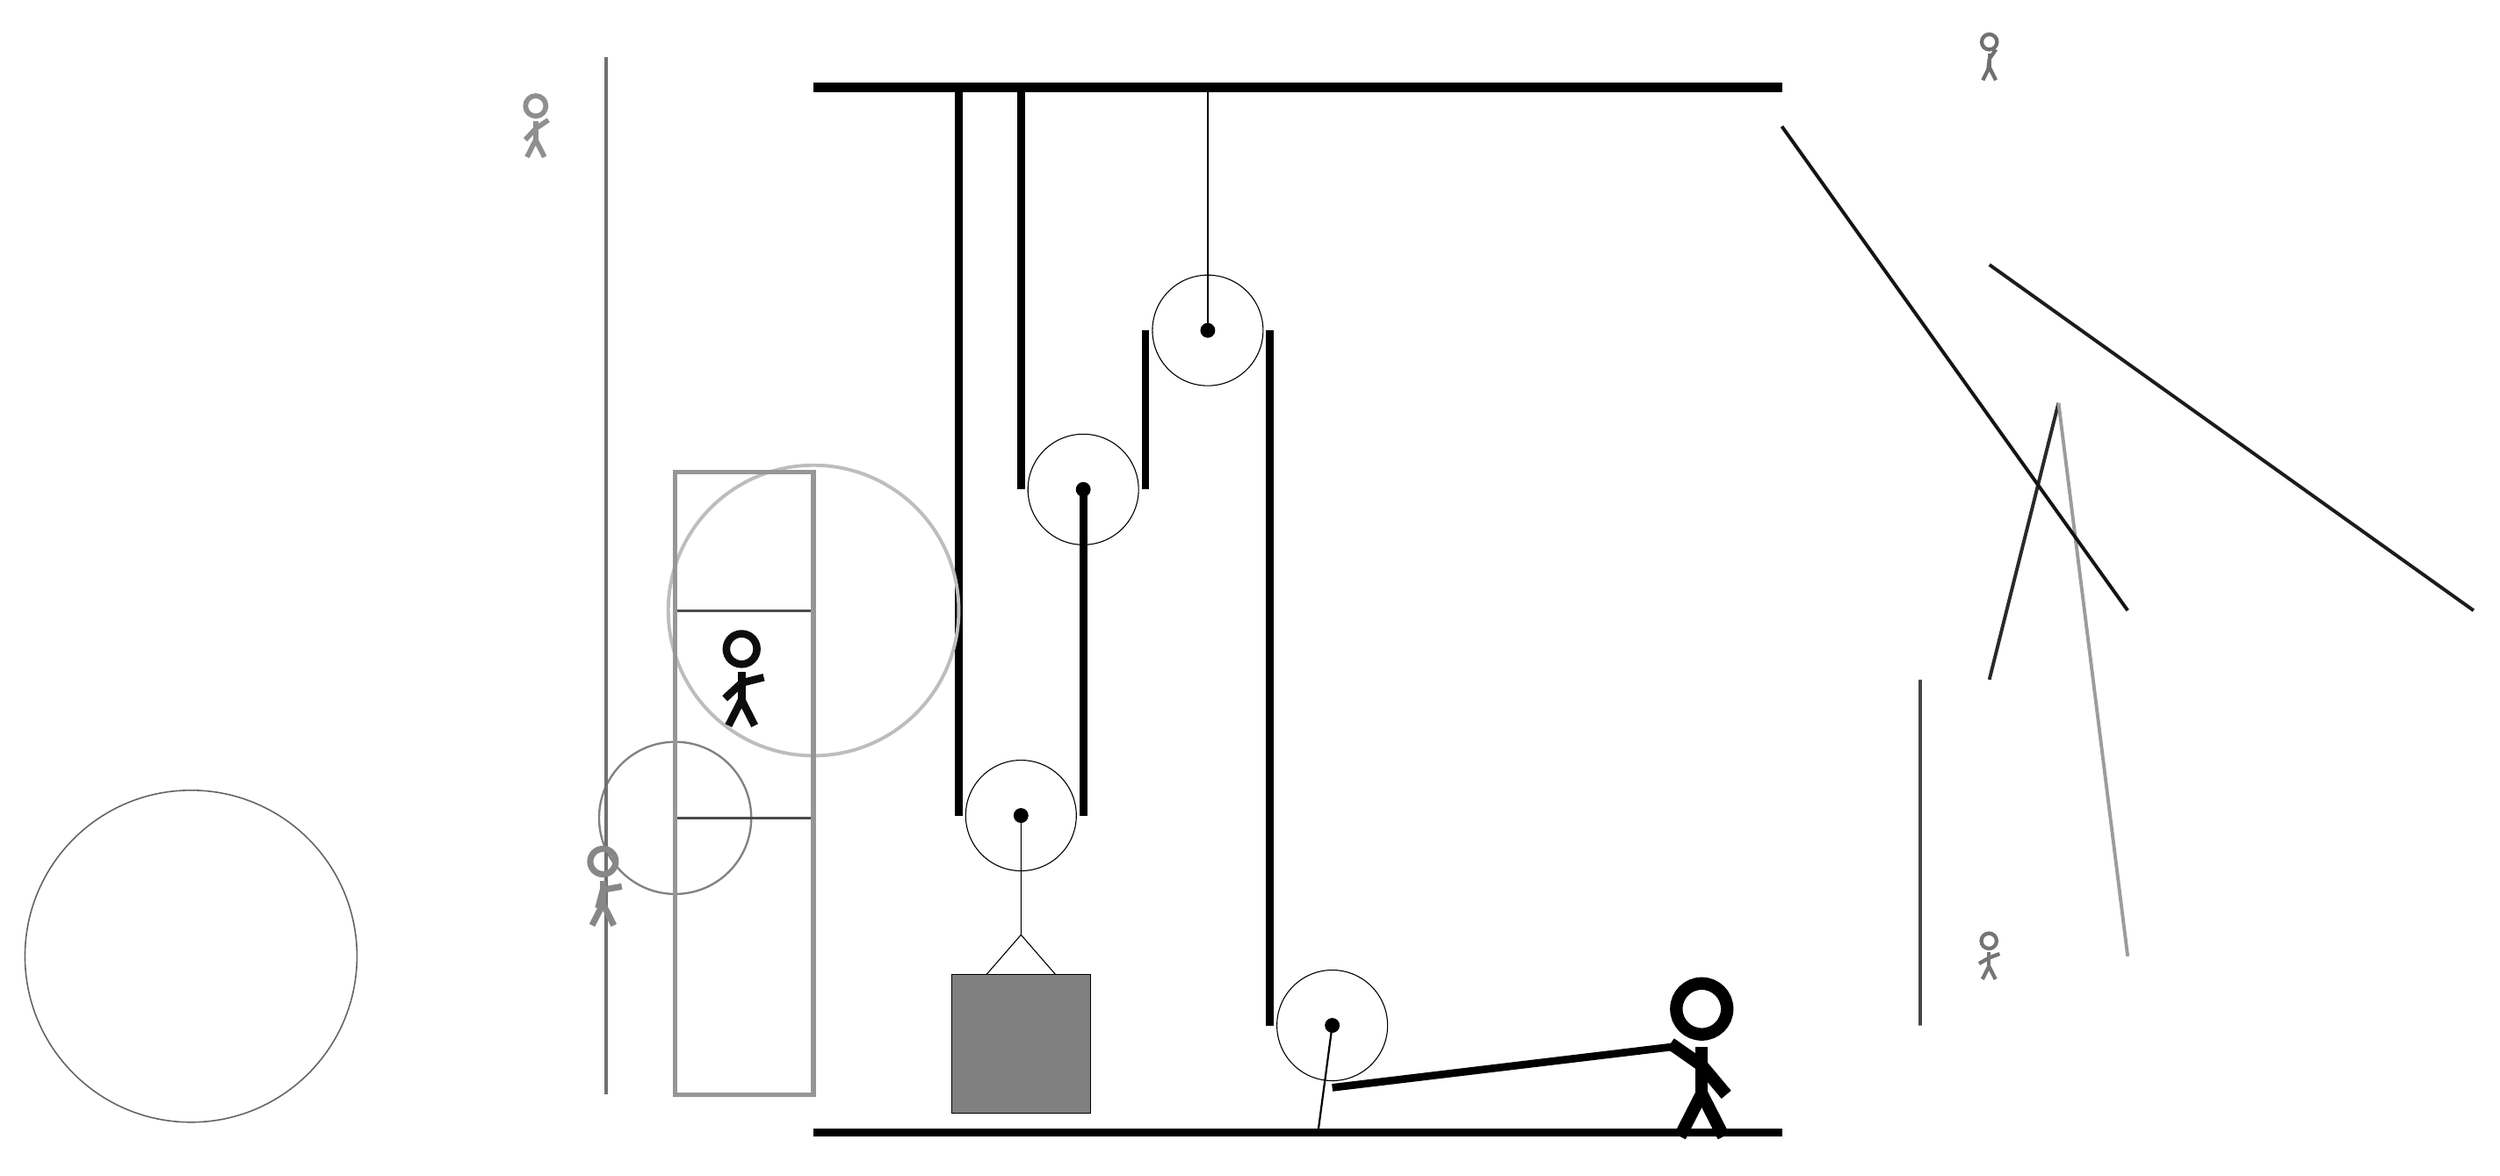
\begin{tikzpicture}
			%%%%% START %%%%%
			
			\draw[fill=black] (-2, 11.5) rectangle (12, 11.625);
			
			\draw (1, 1.035) circle (0.8);
			\draw[fill=black] (1, 1.035) circle (0.1);
			
			\draw (1.9, 5.75) circle (0.8);
			\draw[fill=black] (1.9, 5.75) circle (0.1);
			
			\draw (3.7, 8.05) circle (0.8);
			\draw[fill=black] (3.7, 8.05) circle (0.1);
			\draw[thick] (3.7, 8.05) -- (3.7, 11.5);
			
			\draw (5.5, -2) circle (0.8);
			\draw[fill=black] (5.5, -2) circle (0.1);
			\draw[thick] (5.5, -2) -- (5.3, -3.5);
			
			\draw (1, 1.035) -- (1, -0.69) -- (0.5, -1.265) -- (1.5, -1.265) -- (1, -0.69);
			\draw[fill=black!50] (0, -1.265) rectangle (2, -3.265);
			\draw[line width=1.1mm] (0.1, 11.5) -- (0.1, 1.035);
			\centerarc[line width=1.1mm](1, 1.035)(180:360:0.9);
			\draw[line width=1.1mm](1.9, 1.035) -- (1.9, 5.75);
			\draw[line width=1.1mm] (1.0, 11.5) -- (1.0, 5.75);
			\centerarc[line width=1.1mm](1.9, 5.75)(180:360:0.9);
			\draw[line width=1.1mm](2.8, 5.75) -- (2.8, 8.05);
			\centerarc[line width=1.1mm](3.7, 8.05)(0:180:0.9);
			\draw[line width=1.1mm] (4.6, 8.05) -- (4.6, -2);
			\centerarc[line width=1.1mm](5.5, -2)(0:90:-0.9);
			\draw[line width=1.1mm](5.5, -2.9) -- (10.5, -2.3);
			
			\draw [line width=0.5mm, color=black!26](-2, 4) circle (2.1);
			
			\draw[line width=0.5mm, color=black!89](15, 9) -- (22, 4);
			\node[line width=0.3mm, color=black!44] at (-6, 11) {\Strichmaxerl[4][47][34]};
			\draw[line width=0.5mm, color=black!84](16, 7) -- (15, 3);
			\node[line width=0.5mm, color=black!95] at (-3, 3) {\Strichmaxerl[6][43][14]};
			\draw [line width=0.3mm, color=black!49](-4, 1) circle (1.1);
			
			\draw[line width=0.4mm, color=black!73] (14, 3) rectangle (14, -2);
			
			\node[line width=0.6mm, color=black!56] at (15, 12) {\Strichmaxerl[3][84][55]};
			\node[line width=0.5mm, color=black!54] at (15, -1) {\Strichmaxerl[3][30][21]};
			\draw[line width=0.5mm, color=black!39](16, 7) -- (17, -1);
			\draw[line width=0.4mm, color=black!70] (-4, 1) rectangle (-2, 4);
			
			\draw[line width=0.7mm, color=black!41] (-4, 6) rectangle (-2, -3);
			\draw[line width=0.5mm, color=black!92](17, 4) -- (12, 11);
			
			\draw[line width=0.5mm, color=black!56](-5, 12) -- (-5, -3);
			\draw [line width=0.6mm, color=black!26](17, 10) circle (0.0);
			\draw [line width=0.2mm, color=black!61](-11, -1) circle (2.4);
			
			\node[line width=0.2mm, color=black!47] at (-5, 0) {\Strichmaxerl[5][75][10]};
			
			
			\node at (10.8, -2.5) {\Strichmaxerl[10][-35][-50]};
			
			\draw[fill=black] (-2, -3.5) rectangle (12, -3.6);
			
			%%%%% END %%%%%
		\end{tikzpicture}
	\end{figure}	
\end{document}